%  Mathpartir --- Math Paragraph for Typesetting Inference Rules
%
%  Copyright (C) 2001, 2002, 2003, 2005, 2015 Didier R�my
%
%  Author         : Didier Remy 
%  Version        : 1.3.1
%  Bug Reports    : to author
%  Web Site       : http://pauillac.inria.fr/~remy/latex/
% 
%  Mathpartir is free software; you can redistribute it and/or modify
%  it under the terms of the GNU General Public License as published by
%  the Free Software Foundation; either version 2, or (at your option)
%  any later version.
%  
%  Mathpartir is distributed in the hope that it will be useful,
%  but WITHOUT ANY WARRANTY; without even the implied warranty of
%  MERCHANTABILITY or FITNESS FOR A PARTICULAR PURPOSE.  See the
%  GNU General Public License for more details 
%  (http://pauillac.inria.fr/~remy/license/GPL).
%
%%%%%%%%%%%%%%%%%%%%%%%%%%%%%%%%%%%%%%%%%%%%%%%%%%%%%%%%%%%%%%%%%%%%%%%%%%%%
%  File mathpartir.tex (Documentation)
%%%%%%%%%%%%%%%%%%%%%%%%%%%%%%%%%%%%%%%%%%%%%%%%%%%%%%%%%%%%%%%%%%%%%%%%%%%%

%times new roman
\documentclass[a4paper]{llncs}
\usepackage[T1]{fontenc}
\usepackage[utf8]{inputenc}
\usepackage{mathptmx}

\usepackage {mathpartir}
\usepackage {listings}
\usepackage {float}
%bolding keyword in source code
\usepackage{courier}
%The \usepackage{courier} in the preamble causes \ttfamily to produce output in %the courier font. Without including this package, you can still use \ttfamily to %get a mono spaced font by including that as part of the basicstyle=... setting.

\usepackage{pxfonts}

\usepackage{parcolumns}

\let\oldnl\nl% Store \nl in \oldnl
\newcommand{\nonl}{\renewcommand{\nl}{\let\nl\oldnl}}% Remove line number for one



%pseudocode for algorithm
\usepackage[noend]{algpseudocode}
\usepackage[linesnumbered,ruled]{algorithm2e}


%\renewcommand*\familydefault{\ttdefault} %% Only if the base font of the document is to be typewriter style
%\usepackage[T1]{fontenc}

\usepackage {array}
\usepackage {url}
%\usepackage {subfig}
%\captionsetup[subfloat]{position=bottom,
%  farskip=10pt,topadjust=0pt,captionskip=10pt,
%  nearskip=10pt,margin=10pt}

\usepackage{caption}
\usepackage{subcaption}%if you wish subgraphs side by side
\captionsetup{compatibility=false}

\usepackage{amssymb}
\usepackage{graphicx}

%searching path for figures
\graphicspath{ {./figures/} }
\usepackage{color}



\usepackage{tablefootnote}
\captionsetup[lstlisting]{position=bottom,font=f}
%\usepackage{courier}



\newif \ifhevea 
%HEVEA \heveatrue
\ifhevea 
\usepackage {hevea}
\fi

\lstset {
	%Formatting for code 
	basicstyle=\fontsize{12}\ttfamily ,
	keywordstyle=\color{black}\bfseries ,
		%/underlined bold black keywords			
    %numbers=left,
    %stepnumber=1,
    showstringspaces=false,
    tabsize=1,
    breaklines=true,
     breakatwhitespace=false,
     captionpos=b,
    	keywords={attribute},
}


\let \lst \verb
%
%\title {
%HEVEA\begin{tabular}{>{\huge}c}
%\textbf{MATH} formulas in \\ 
%\textbf{PAR}ragraph mode\\[-1ex]
%\ifhevea\else{}\hskip 0em\hbox to 12em {\hrulefill}\\\fi
%HEVEA\hline
%\textbf Typesetting \textbf Inference \textbf Rules \\
%HEVEA\end{tabular}
%}


\title {Enabling pointers in automatic program separation}




%\author {Didier R{\'{e}}my}
\author {}

\date {(Version 1.5, last modified 08/10/2016)}


\begin{document}

\maketitle

\begin{abstract}

This is abstract.
%%Type conversion between C and protocol buffer is an important issue in our project. When the separation is done and the RPC tool begins working, we must automatically restore all the arguments for each RPC function in the receiver process, which means the function parameter types need to be transmitted between two processes fully and exactly. Unfortunately, the type system that protocol buffer supports is quite weak. To make our project automatically run in the end, we have to design a type conversion protocol to let protocol buffer automatically convert some advanced C types(e.g. pointer) into protocol buffer types. 

\end{abstract}


\section {Introduction}

We proposed a type-based approach that can automatically separate one program into two modules that can run separately.\\

Contribution: previous works do not solve the pointer issues well, we do. \\


\section {Related work}


\section {Separation Framework}
\subsection {Program dependence graph}

Program Dependence Graph(PDG) plays a key role in our separation framework. We develop a toolchain which can build instruction-grained PDGs for LLVM IRs. Our toolchain wraps up each IR instruction as a graph node, and adds some auxiliary data nodes to help represent the inter-procedural dependences. So, we have two kinds of node in a PDG:\\

(1) \textbf{instruction nodes}: an instruction node is used to represent an LLVM IR instruction;\\

(2) \textbf{data nodes}: used to represent: (1) global values; (2) auxiliary trees that called \textit{parameter trees} for representing the parameter passing. \\




%(3) \textbf{parameter tree node}: used to build the parameter trees.\\

Accordingly, we have four kinds of edges:\\

(1) \textbf{control dependence edges}: used to represent a control dependence;\\

(2) \textbf{data dependence edges}: used to represent a data dependence;\\

(3) \textbf{parameter tree edges}: used to connect the corresponding data nodes to form a parameter tree that represents a function parameter or a global variable;\\

(4) \textbf{call edges}: used to connect the call site with the entry site of callee function. For indirect calls, we use a type-based approximation to connect the call site with all possible target callees with the same type.\\ 

Topologically, a PDG for a program with multiple functions is an inter-procedural extension of a program with only one function. So, accordingly, to build a PDG for a large program with multiple functions, we build a PDG for each function first, and then "glue" these small PDGs together. In other words, we first model all the intra-procedural dependences. Then, based on the caller-callee relationships, we build the corresponding \textit{parameter trees}\cite{interslicing} to model the inter-procedural dependences. We also use the parameter trees to represent the global data structures, and construct the data dependences between the global variables and their caller functions. The benefits of using the parameter trees are: (1)we can clearly represent the memory layout of the function parameters(or global variables) with pointers;(2)we can easily represent the data flows in a parameter passing process between a caller function and a callee function;
(3)we can construct the PDG modularly and accurately.



\subsubsection{Modeling intra-procedural dependences}
The intra-procedural dependences consist of both control dependences and data dependences. The control dependences within a function can be captured easily with the classical post-dominator-tree-based algorithm\cite{ferrante}. Computing the data dependences is a little harder since we need to process two different kinds of data dependences separately. They are:\\

\textbf{definition-use dependence}: Given two instructions $I_d$ and $I_u$, if a variable is defined in $I_d$, and then used in $I_u$, then we say there is a definition-use data dependence from $I_d$ to $I_u$, noted as $I_d \rightarrow I_u$.\\ 

\textbf{flow dependence}: Given two instructions $I_r$ and $I_w$, if $I_r$ reads memory that was written by $I_w$ (RAW: read after write), then we say there is a flow dependence from $I_w$ from $I_r$, noted as $I_w \rightarrow I_r$.\\

An example of two kinds of data dependences is listed in Fig.1.\\

% the \textbf{def-use dependences} and the \textbf{flow dependences}(\textbf{true data dependences}). The def-use dependence represents the data dependency between two statements with the definition-use association(DUA,see Fig 1.a), and the flow dependence represents the dependency between memory read and write operations(read-after-write,see Fig 1.b). In this paper, both the \textbf{anti-}dependence (write-after-read) and the \textbf{output-}dependence(write-after-write) are not in our consideration, and we only compute the flow dependence.\\

%
%\begin{figure}[ht!]
%    \centering
%        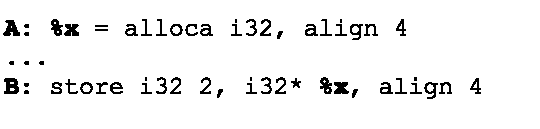
\includegraphics[height=0.7in, width=2.8in]{def-use.pdf}
%   
%        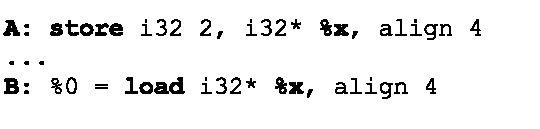
\includegraphics[height=0.7in, width=2.8in]{flow-dep.pdf}
%
% 
%    \caption{An example of two kinds of data dependences}
%    %\label{figure 1}
%\end{figure}


\begin{figure}[ht!]
    \centering
    \begin{subfigure}[t]{0.5\textwidth}
        \centering
        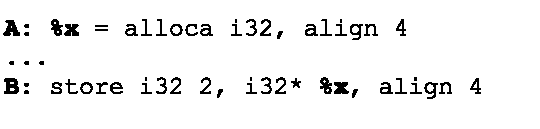
\includegraphics[height=0.7in, width=2.8in]{def-use.pdf}
        \subcaption{a def-use dependence $A \rightarrow B$}
    %    	\label{def-use}
    \end{subfigure}
    ~
    \begin{subfigure}[t]{0.5\textwidth}
        \centering
        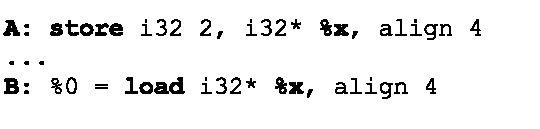
\includegraphics[height=0.7in, width=2.8in]{flow-dep.pdf}
        \subcaption{a flow dependence $A \rightarrow B$}
    %    	\label{flow-dep.pdf}
    \end{subfigure}
    \caption{An example of two kinds of data dependences}
    %\label{figure 1}
\end{figure}





The definition-use dependences can be detected easily because LLVM uses the SSA form. So, in order to detect a definition-use data dependence, it suffices to retrieve each operand in an instruction $I_u$, and add a dependence from the instruction $I_d$ that defines this operand to $I_u$.\\ 


%by finding all variables in an IR instruction and then adding a dependence between it and the statement that defines the variable.

In LLVM, only \texttt{store} instructions can write data into memory and only \texttt{load} instructions can read data from memory. By our definition, clearly the flow dependencies in LLVM only exist between the \texttt{store} instructions and \texttt{load} instructions. So, our algorithm for computing all of intra-procedural flow dependencies can be described as follows:\\

In procedure \textit{P}, for each \texttt{load} instruction $l_i$, check each \texttt{store} instruction $s_i$ in \textit{P}, if $l_i$ and $s_i$ access the same memory location (e.g. \texttt{\%x} in Fig.1 (b)), $s_i \rightarrow l_i$ is a flow dependence. Clearly we make an approximation here since we ignore considering the sequence of the \texttt{store}/\texttt{load} instructions, which may lead to some redundant dependences being added.\\

Besides, an alias analysis step is required in finding the flow dependences. In our work, we use the DSA algorithm\cite{dsa} to help compute the aliases because it is a kind of open-source, context-sensitive and field-sensitive algorithm that can be applied to large server applications\cite{jujutsu}.\\

Once we finished constructing the PDG for each procedure, we can start to model the inter-procedural dependences to construct the PDG for the whole program.

\subsubsection{Modeling inter-procedural dependences}

The inter-procedural data dependency fully depends on the function parameter passing. So, the core part of modeling inter-procedural data dependency is how to represent the data dependency between the \textbf{actual parameters (arguments)} and the \textbf{formal parameters}. To achieve the field-sensitivity and represent the data layout of parameters in memory as precisely as possible, we use trees to model function parameters. In this paper, these trees are called \emph{parameter trees}. \\

Once we construct the parameter trees for a parameter $p$, we can clearly represent the field-sensitive data flow in $p$'s parameter passing by connecting its corresponding tree nodes. If $p$ is a pointer, we need to further model the dependency associated with the value that $p$ points to.\\

We model 4 parameter trees for each parameter in total. They are:\\

\textbf{actual-in tree}: used to represent a new actual parameter before entering the callee function;\\

\textbf{actual-out tree}: used to represent the modified actual parameter when a call is finished;\\

\textbf{formal-in tree}: the callee analog of actual-in tree, used to represent the formal parameter before the callee execution;\\

\textbf{formal-out tree}: the callee analog of actual-out tree, used to represent the modified formal parameter after the callee execution.\\

For each function\footnote{Library functions(e.g.\emph{scanf}, \emph{printf}, \emph{exit}...) will not be unfolded as subgraphs but represented as common nodes instead.} \textit{f}, we only need to build its formal-in and formal-out trees once because \textit{f} only has one function body. On the other hand, the number of actual-in and actual-out trees depends on how many calls we have in a program. If \textit{f} is directly called by another function \textit{q}, we build the actual-in and actual-out trees at the call site, which is within \textit{q}. So, each direct call for \textit{f} matches exactly one pair of formal-in and formal-out trees.\\

As we mentioned before, using parameter trees can show the memory layout of variables very clearly. Each node in a parameter tree actually represents a piece of abstract memory whose size corresponds to the type associated with the node. Our algorithm for modeling a function parameter $p$'s parameter tree is shown in Algorithm 1. The algorithm is fully based on $p$'s type, noted as \textit{type(p)}. First, we take \textit{type(p)} as the tree root, if it is a basic type\footnote{In C, this means types formed by four basic type specifiers \emph{char}, \emph{int}, \emph{float}, \emph{double} and four modifiers \emph{signed}, \emph{unsigned}, \emph{short} and \emph{long}.}, we leave \textit{type(p)} as a single leaf node and stop, and in this case all $p$'s parameter trees shrink to single nodes accordingly; if \textit{p} is a pointer, we insert \textit{type(*p)} into the tree as the only child of \textit{type(p)} and process \textit{type(*p)} to build subtrees recursively; if \textit{type(p)} is a structure type, we retrieve each field $f_{i}$ in \textit{p} and insert \textit{type($f_{i}$)} as a child of \textit{type(p)}, and then use \textit{type($f_{i}$)} as the input to build a subtree. In Fig.2, we use a typical structure type to show how a type-based parameter tree looks like. \\

\begin{figure*}[ht!]
    \centering
    \begin{subfigure}[ht]{0.5\textwidth}
        \centering
        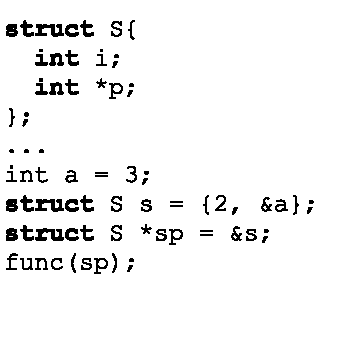
\includegraphics[height=1.5in]{parameter-tree-code.pdf}
        \subcaption{\texttt{sp}: a pointer which points to a structure}
    \end{subfigure}%
    ~ 
    \begin{subfigure}[ht]{0.5\textwidth}
        \centering
        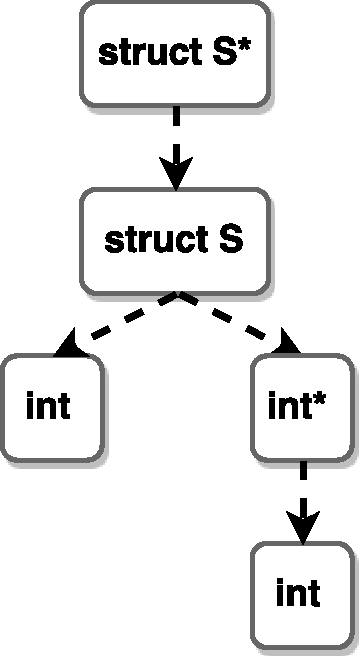
\includegraphics[height=1.5in]{parameter-tree-graph.pdf}
        \subcaption{the type-based parameter tree of \texttt{sp}}
    \end{subfigure}
    \caption{Example: a type-based parameter tree}
\end{figure*}






% Each incoming parameter \textit{p} corresponds to a root. If \textit{p} is a pointer, we insert the value that \emph{p} points to into the tree as the only child of \textit{p} and process this value to build subtrees recursively; otherwise if \textit{p} is a struct, we retrieve each field $f_{i}$ in \textit{p} and insert $f_{i}$ as a child of \textit{p}, and then use $f_{i}$ as input to build a subtree; if \textit{p} is neither a pointer nor a struct, which means it must be a variable of base type\footnote{For simplicity, we take \texttt{string} as an atomic type also.}(e.g. int, float, char...), \textit{p} will be inserted as a leaf. Actually the parameter tree for an atomic variable always shrinks to a single node. An example of parameter tree\\


\begin{algorithm}[!h]

	\nonl Parameter type $t$ := $base\ type$ | $t^{'}*$ | $struct\ \{t_1;\ t_2;\ ...\ ;\ t_n\}$.\\
	%| $type\_name\  S$
	\nonl $appendSubtrees(root,\ t_1,\ t_2,\ ...\ ,\ t_n)$ : append trees $t_1$, $t_2$, ... , $t_n$ as the children of $root$ .\\
	\\

	\State $buildTree (t)$\\ 

\Switch{t}{

	\Case{$t^{'}*$}{
		\State let $subtree = buildTree(t^{'})$  in $appendSubtrees(t,\ subtree);$\\
	}

	\Case{$struct\ \{t_1;\ t_2;\ ...\ ;\ t_n\}$}{
		\State let $subtree_1 = buildTree(t_1)$  in\\
		\State let $subtree_2 = buildTree(t_2)$  in\\
		\State ...\\
		\State let $subtree_n = buildTree(t_n)$  in $appendSubtrees(t,\ subtree_1,\ subtree_2,\ ...\ ,\ subtree_n);$\\
	}
%	\tcc{atomic parameter}
	\Other(\tcc*[h]{t is a base type}){ 
	
		\State $appendSubtrees(t,\ null);$   \tcc{Leave t as a leaf node}\\
		
	}
}
%    \SetKwInOut{Input}{Input}
%   \SetKwInOut{Output}{Output}

%	\State $BuildTree (t)$\\
%    \Input{$p$-- parameter; $T$-- a pointer which points to the tree root }
%    \Output{a constructed tree represented by $T$}
%
%	\State $T \rightarrow root = p$;
%
%    \eIf{$p$ is a pointer}
%      {
%		\State $T->root = p$; 	       	
%      	\State $T \rightarrow root \rightarrow firstchild = dereference(p)$
%      	\tcc*[r]{insert *p}
%      	\State $BuildTree(dereference(p), T \rightarrow root \rightarrow firstchild);$
%      }
%      {
%        \eIf{$p$ is a struct}
%      	{
%      		\State $T->root = p$;
%	      	\For{each field $f_{i}$ in $p$} 
%	      	{
%	 	 	   	\State $T \rightarrow root \rightarrow appendchild(f_{i})$;	
%	 	 	    \State $BuildTree(f_{i}, T \rightarrow root \rightarrow getchild(i));$
%	      	} 
%			\EndFor
%      	}
%      	{ %atomic parameter
%      	\tcc*{atomic parameter}		      		
%      	}
%
%      }
    \caption{building a parameter tree}
\end{algorithm}


One problem about representing parameters with tree structures is some parameters may have recursive data structures(e.g. linked list) that can lead to parameter trees of infinite depth. In our framework, we use the $k-$limiting approach\cite{k-limit} to forcibly expand the tree to level $k$ only to prevent infinite expansions. For simplicity, we let $k$=$1$. An example of building a $1-$limiting parameter tree for a recursive data structure is listed in Fig.3. \\


%To solve this problem Graf\cite{objectgraph} proposes an algorithm to unfold the recursive data structures. 


\begin{figure*}[!ht]
    \centering
    \begin{subfigure}[ht]{0.5\textwidth}
        \centering
        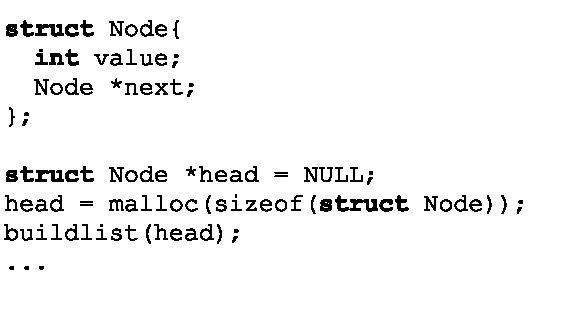
\includegraphics[height=1.5in]{recursive-code.pdf}
        \caption{a linked list program}
    \end{subfigure}%
    ~ 
    \begin{subfigure}[ht]{0.5\textwidth}
        \centering
        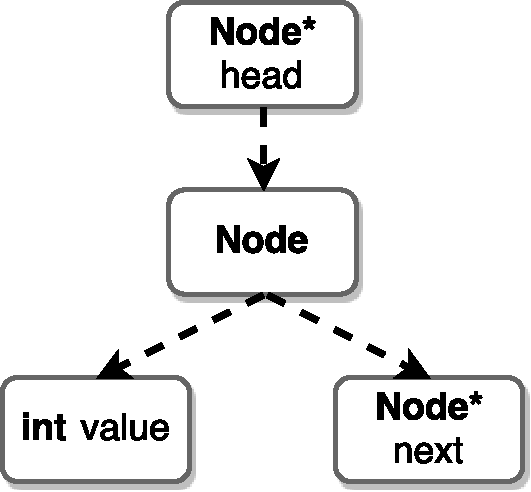
\includegraphics[height=1.5in]{recursive-tree.pdf}
        \caption{an unfolded parameter tree}
    \end{subfigure}
    \caption{An example of parameter trees with recursive data structure}
\end{figure*}


We also use the tree data structure to model the global variables for better field-sensitivity. The algorithm for building the global variable trees is completely the same as building the function parameter trees.

\subsubsection{indirect function call}


If a function \textit{f} is called indirectly, it is impossible for us to exactly locate the position of callee function. Our solution is to approximately retrieve all possible candidate functions with the same type as \textit{f} and build actual-in/out trees for each of them. Considering this is still a type-based matching, we have to do some preprocessing to guarantee that in the input programs for separation we have (1) no type cast to or from function pointer types and (2) no assembly code. This preprocessing is necessary because both of the two cases will lead to the failure of our type-based indirect call matching. While once we finished the preprocessing, this type-based indirect call matching is compatible with the parameter trees construction.


%which means some redundant actual trees will be built inevitably
\subsubsection{Example: encrypt a password}

Let us see a real example. The toy program in Figure 4 includes a function with simple greeting, a function for password encryption and the main function. In line 2, we mark array \texttt{password} as a piece of sensitive data. Figure 3 is the PDG model for this toy program. We omit most of the simple intra-dependences, and only keep the most interesting part about how to use parameter trees to represent the inter-procedural data dependency.\\
\begin{figure}
\begin{lstlisting}[h, language=C, basicstyle=\fontsize{12}\ttfamily, numbers=left, stepnumber=1]
static char username[20];
static char __attribute__(sensitive) password[20];  

int greeter(char *str){
  if(str == NULL) 
  	return 1;
  printf("Welcome %s!"\n, str);
  return 0;
} 

int encrypt(char *str,int key){
  unsigned int i;
  for(i = 0; i < strlen(str); ++i){
    str[i] = str[i] - key;
  }
  return 0;
}
 
int main(){
  printf("Create your username: \n");
  scanf("%s", username);
  if(greeter(username) == 1)
    printf("Invalid user!\n");
  printf("Enter your password: \n");
  scanf("%s", password);
  printf("password:%s\n", encrypt(password,5));
  return 0;
}

\end{lstlisting}
\caption{A toy C program to encrypt a password.}
\end{figure}

\begin{figure}[!htb]
	\centering
	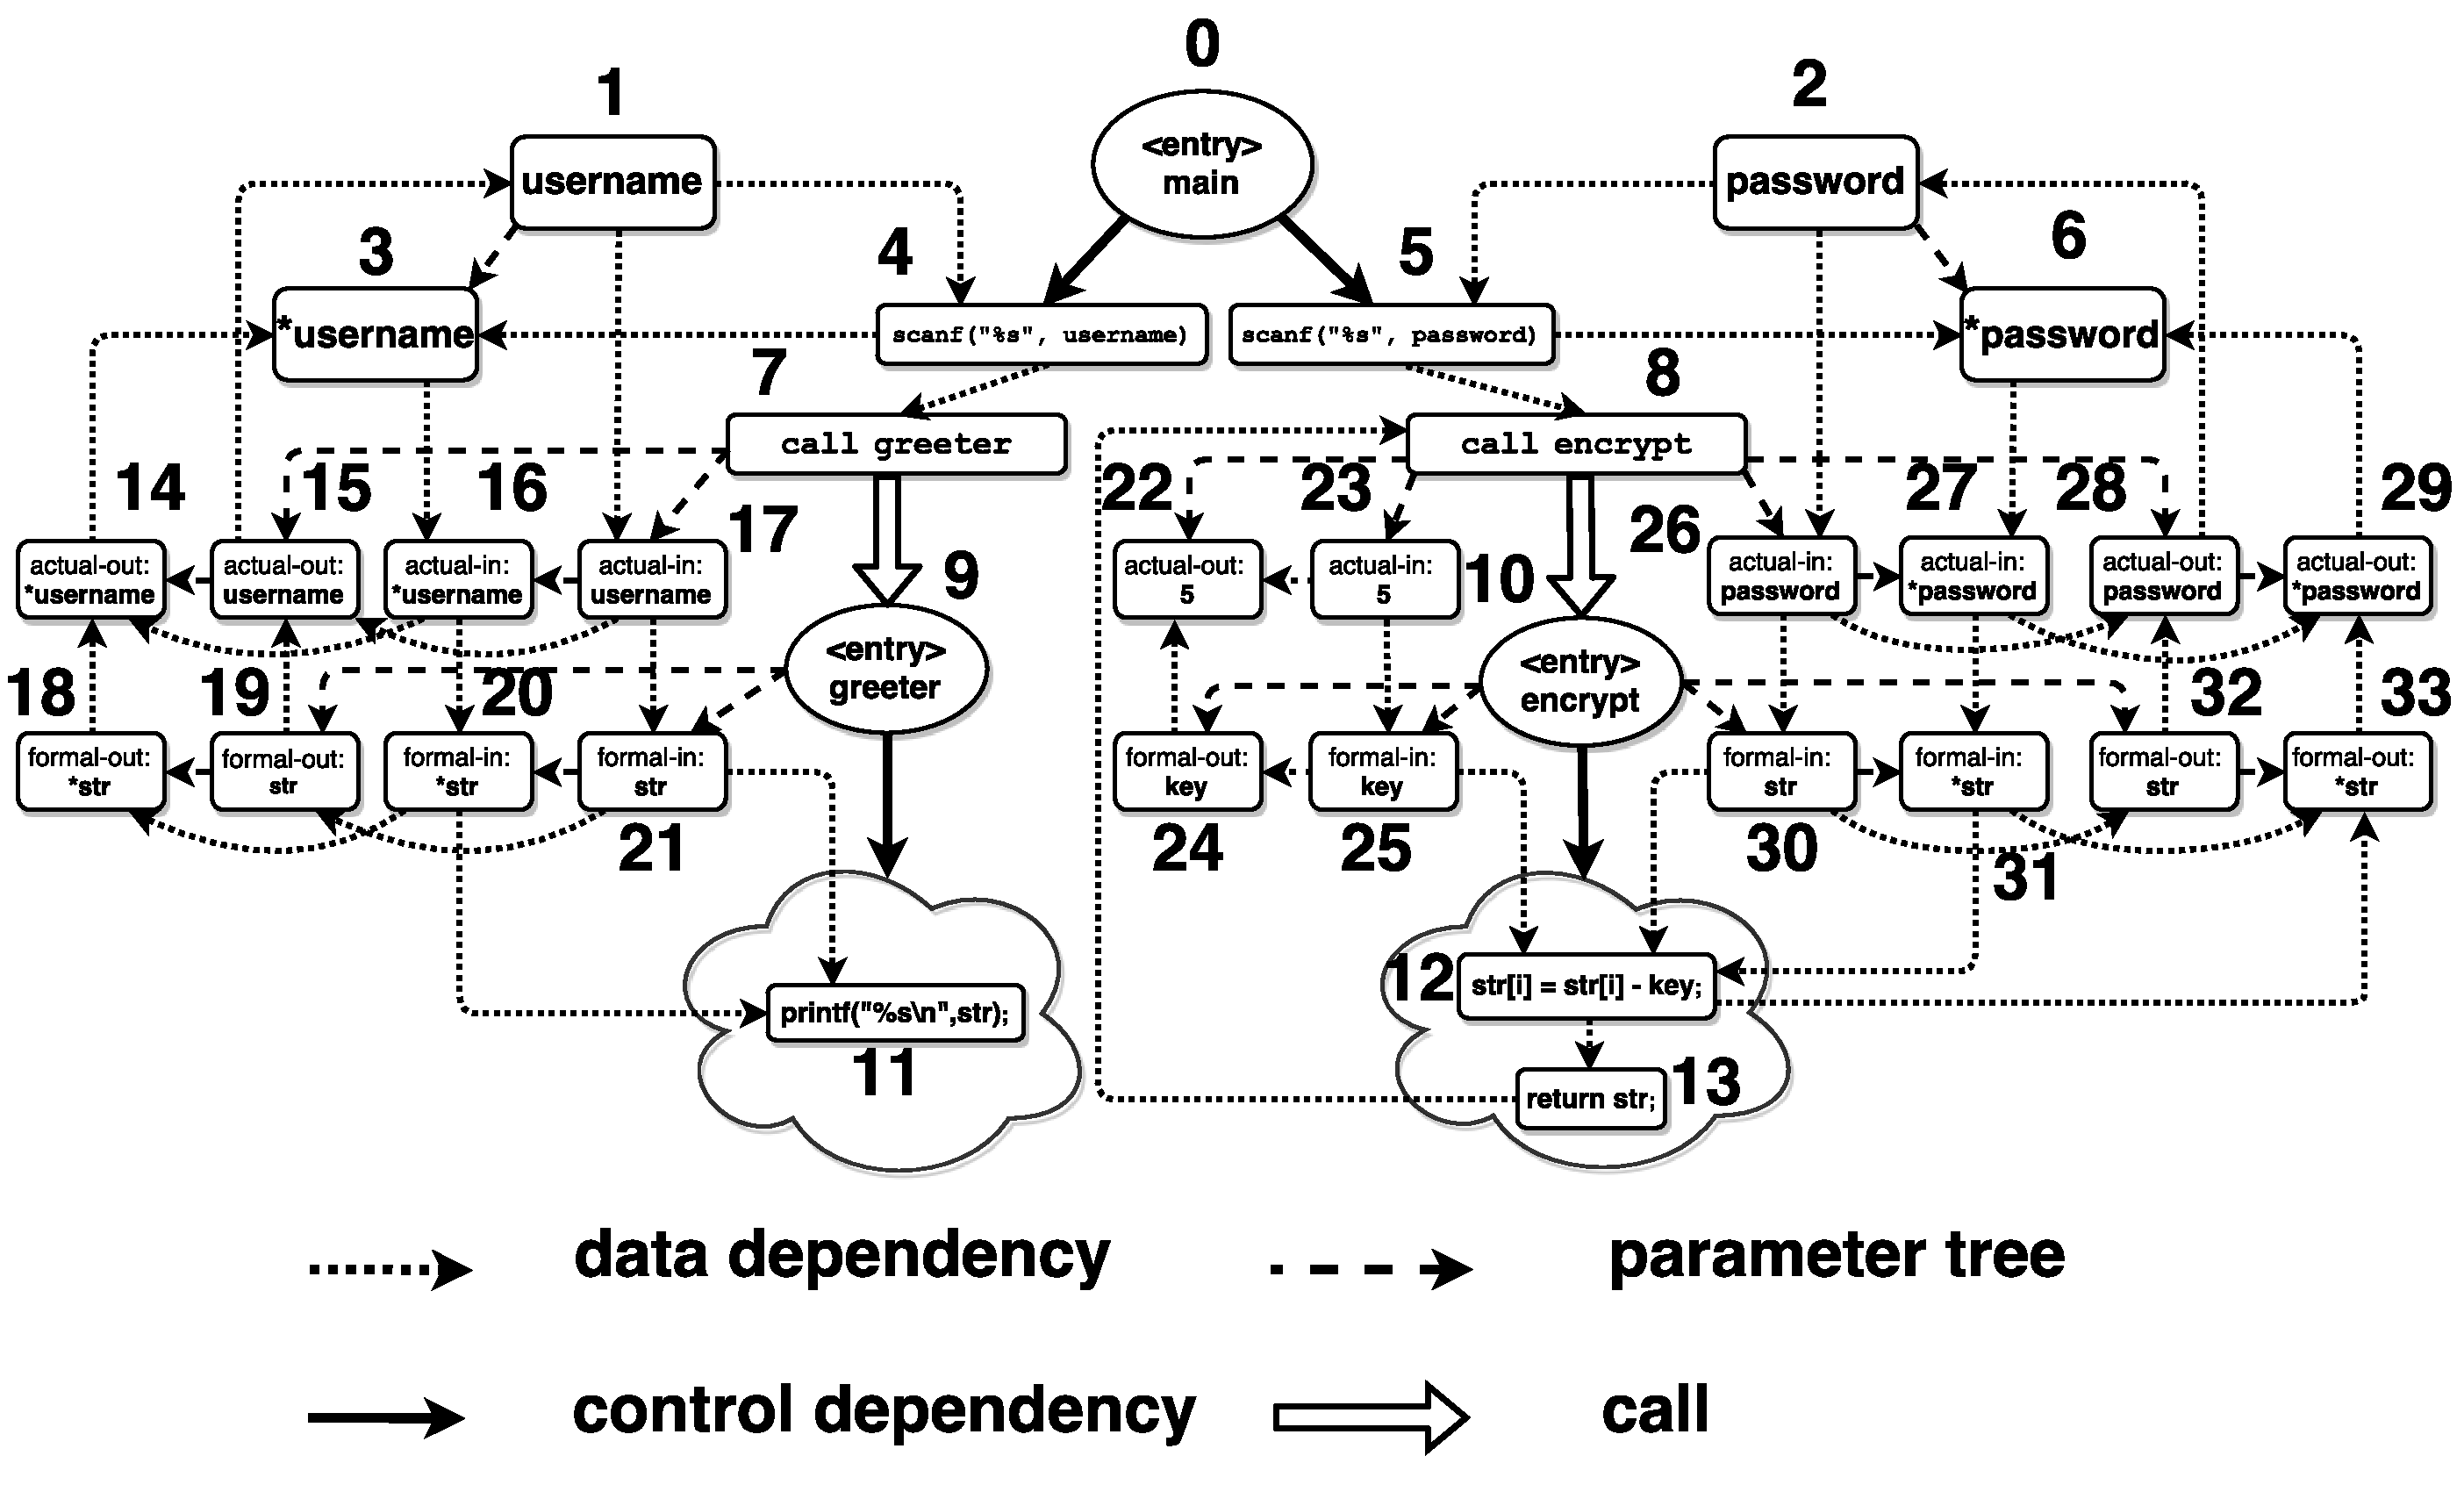
\includegraphics[width=\textwidth]{PDG.pdf}
	%\vspace{-0.15in}
	\caption{The program dependence graph of our toy program.}
	\label{fig:daemon}
	%\vspace{-0.2in}
\end{figure}


In Figure 5, we construct two trees for global arrays \texttt{username} and \texttt{password} separately. Considering all arrays passed to functions are converted into pointers in C, we directly represent them with the form of \texttt{char*} instead of \texttt{char[]}, and by doing this we can show the data dependency better. As you can see on the upper-left part, node 1, which is the root of the global variable tree for \texttt{username}, represents the pointer that points to the username string; while node 3 represents the content that pointer points to, i.e., the string itself. By algorithm 1 clearly node 3 is the child of node 1, and also a leaf since we take \texttt{string} as an atomic type just as we mentioned before. In the main function, we need to set up a def-use data dependence edge $(1 \rightarrow 4)$, and a flow dependence data dependence edge $(4 \rightarrow 3)$ since the operation \texttt{scanf} uses the pointer "username" first and then modifies the value that pointer "username" points to.\\ 

Next, we have a data dependence edge $(4 \rightarrow 7)$ because we take the call operation(node 7) as a kind of use of "username". We use a call edge$(7 \rightarrow 9)$ to connect the call site(node 7) in the caller function(\texttt{main}) and the entry node of the callee function(\texttt{greeter}). The function body of \texttt{greeter} is abstracted as a cloud-like region, connected with its entry node through an abstract control dependence edge $(9 \rightarrow 11)$.


Now we can use parameter trees to represent the parameter passing between \texttt{main} and \texttt{greeter}. We let the call node(node 7) dominate the actual-in(node 16, node 17) and actual-out(node 15, node 14) trees,and the entry node of greeter(node 9) dominate the formal-in(node 21 and 20) and formal-out(node 19 and 18) trees. There are two kinds of data flow when the parameter is a pointer: one is the data flow of the pointer itself, and the other is the data flow of the value that pointer points to(pointee). On this graph, the data flow of the pointer itself(username) can be represented by a node sequence $1 \rightarrow 17 \rightarrow 21 \rightarrow 19 \rightarrow 15 \rightarrow 1$, which is a loop actually. Accordingly, the data flow of the pointee of "username" can be represented with the sequence $3 \rightarrow 16 \rightarrow 20 \rightarrow 18 \rightarrow 14 \rightarrow 3$. However, there is only memory read(node 11) but no write operation in function greeter, so we only have two data dependence edges ($21 \rightarrow 11$) and ($20 \rightarrow 11$), which both come from the caller to callee. 

The PDG construction for \texttt(encrypt) is similar. The first parameter is just an integer so each parameter tree is simply constructed as a single node. There is a data dependence edge ($25 \rightarrow 12$) since the formal parameter "key" is read by statement "\texttt{str[i] = str[i] - key;}". One important data dependence edge in \texttt{encrypt} is ($12 \rightarrow 33$), which represents that we update the buffer that the pointer "str" points to inside the callee function. Finally, we have a a data dependence edge ($13 \rightarrow 8$) to represent the data flow of return value.\\



\subsection {PDG-based separation algorithm}


After we have a PDG for a program, we can separate this program into two slices by partitioning its PDG into two cuts. Simply speaking, we first annotate some sensitive data in the program with the \texttt{\_\_attribute\_\_} grammar(see line 2 in Figure 4) and take the corresponding graph nodes as the source, and then start from the source nodes to do a greedy coloring along the data dependence edges on the graph. After the coloring finished, we get two sets of graph nodes, one consists of all the colored nodes and the other consists of all the uncolored nodes. In the set of the colored nodes, we check each node one by one, if it corresponds to a global variable, we directly mark that global variable as sensitive, and if it corresponds to a statement within a function, we mark that function as sensitive. Ultimately, all the sensitive functions and global variables will be separated from the original input program as an independent slice, and we call this slice a "sensitive slice". On the other hand, the left global variables and functions that are non-sensitive form another slice, and we call it "non-sensitive slice" accordingly. A detailed description of our separation is in Algorithm 2.\\


\begin{algorithm}[H]
    \SetKwInOut{Input}{Input}
    \SetKwInOut{Output}{Output}

	\State $Program\_Separate (PDG,\ function\_set,\ global\_set,\ source\_nodes,\ colored\_nodes,\ Queue)$\\
    \Input \noindent\nonl{$PDG(N,E)$ --- a directed graph which represents the whole input program $P$, where $N$ is the set of nodes and $E$ is the set of edges;\\ $function\_set$ --- a set which contains all the functions in $P$;\\ $global\_set$ --- a set which contains all the global variables in $P$;\\ 

%$sensitive\_function\_set$ --- a set which contains all the sensitive functions after separation;\\
%$sensitive\_global\_set$ --- a set which contains all the sensitive global variables after separation;\\    
    $source\_nodes$ --- a set which contains all the nodes that marked as "sensitive" on the PDG;\\ $colored\_nodes$ --- a set which contains all the colored graph nodes during the coloring};\\ $Queue$ --- a priority queue used for the greedy graph coloring;\\
    
    \Output \noindent\nonl{$function\_set$ --- a set with all sensitive functions colored and non-sensitive functions uncolored;\\ $global\_set$ --- a set with all global variables colored and non-sensitive global variables uncolored}.

	\State $Initialization:$
	\State $colored\_nodes \leftarrow source\_nodes$;
	\State $current\_node \leftarrow NULL$ 	
	\tcc*[r]{the node we are working on}
%	\State $sensitive\_function\_set \leftarrow NULL$ 
%	\State $sensitive\_global\_set \leftarrow NULL$ 


	\ForEach{node n in source\_nodes}
		{
			\State $Push(Queue,\ n)$;
			\State Color $n$;
			\State $Insert(colored\_nodes,\  n)$;
		}

	\While{Queue is not empty}
		{
			\State $current\_node \leftarrow Pop(Queue)$;\\
			\ForEach{successor node $n_s$ of $current\_node$}
				{

					\If{$s_n$ is uncolored {\bf and} $(n \rightarrow n_s)$ is a data dependence edge}
						{
							\State Color $n_s$;
							\State $Insert(colored\_nodes,\  n_s)$;		
							\State $Push(Queue,\  n_s)$;					
						}
				}  
		}

	\ForEach{node c in colored\_nodes}
		{
			\State Color c's corresponding function $f_c$ in $function\_set$;
	%		\State $Insert(sensitive\_function\_set,\ f_c)$;
			\State Color c's corresponding global variable $g_c$ in $global\_set$;
	%		\State $Insert(sensitive\_global\_set,\ g_c)$;
		}
    \caption{PDG-based program separation}
\end{algorithm}




\section {Inter-module communication after separation}

\subsection {Basic workflow}


The slices we have by the graph-based separation algorithm above are just two sets of functions and global variables. We call these slices "\textit{raw slices}" because these code can not be executed directly for missing the necessary context. For example, in the above encryption program, if we want to run the sensitive slice with function \textit{encrypt} and \textit{main}, we will be stuck at line 21 and 22 since the variable \textit{username} and function \textit{greeter} are defined in another slice.\\

Clearly, our goal of doing program separation is not only to generate some raw slices but also to make these slices can run as real modules, and then we can use other techniques to protect those sensitive modules specially. So, once we successfully separate a program into two raw slices, we need to wrap up each raw slice with some context wrapper functions to make it become a module that can run independently. Further, we can use RPC (Remote Procedure Call) to accomplish the inter-module communication to make the new modular program work well as if it has never been separated before.\\ 

\begin{figure}[!htb]
	\centering
	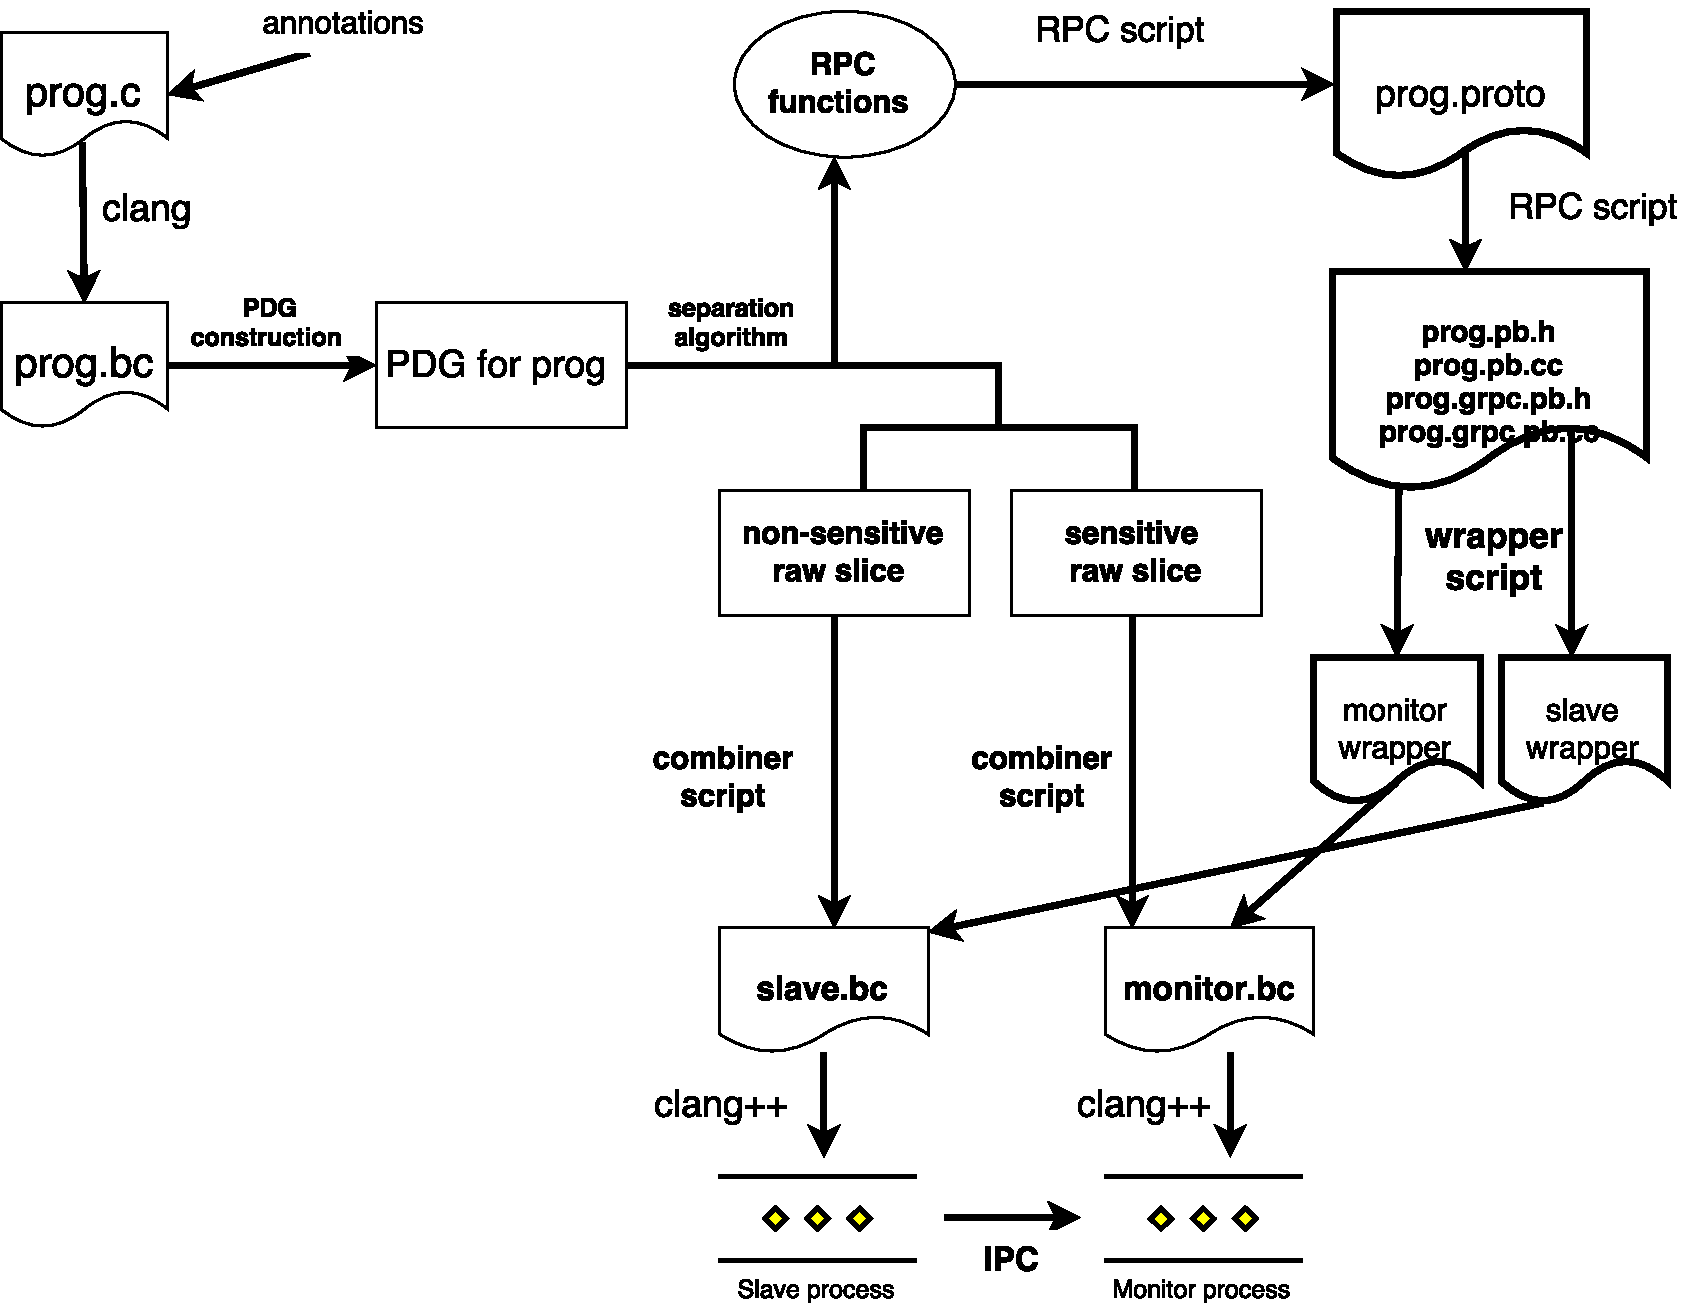
\includegraphics[width=\textwidth]{separation-flow.pdf}
	%\vspace{-0.15in}
	\caption{the automatic program separation framework}
	\label{fig:daemon}
	%\vspace{-0.2in}
\end{figure}


We show the whole working process of our separation framework in  Fig.6. At the beginning, we add some annotations in the input C program noted as \texttt{prog.c}, and then compile the annotated C program into an LLVM IR file noted as \texttt{prog.bc}. Then, we construct the program dependence graph for \texttt{prog.bc}. By our separation algorithm, we can separate \texttt{prog.bc} into two raw slices, one is sensitive while another is non-sensitive. During the separation process, we record all the functions that need to be called remotely by the RPC framework in future, and automatically generate a bunch of interface files with our RPC scripts. Based on these generated interface files, we can use a wrapper script to generate two wrapper files of LLVM IR form, noted as the monitor wrapper and the slave wrapper separately. Next, we use a combiner script to link the monitor wrapper and the sensitive raw slice to get a runnable new IR called \texttt{monitor.bc}, and link the slave wrapper and the non-sensitive raw slice to get an IR called \texttt{slave.bc}. Finally, we compile \texttt{monitor.bc} and \texttt{slave.bc} with clang++ to create two processes, one is called slave and the other is called monitor. The inter-process communication between the slave process and the monitor process is also implemented by our RPC framework.\\


\subsection {RPC framework}

\subsubsection {gRPC}

We use gRPC, a RPC library that is fully based on google protocol buffer, to deal with the RPC issues in our work. In gRPC, a C type must be packed to a protocol buffer type of form ``\texttt{message}'' in a .proto file for further transmission. For example, if we have a C function \texttt{int foo(int x)} which needs to be called remotely, then in the .proto file, the argument type \texttt{int} can be packed in protocol buffer as follows:\\

\begin{lstlisting}[xleftmargin=.1\textwidth] 
message M{                    message M{
  int64 x=1;      or            int32 x=1
}                             }

\end{lstlisting}

Next, protocol buffer will automatically generate a group of read/write APIs for each message. Here is an API for x's value assignment:  

\begin{lstlisting}[xleftmargin=.1\textwidth]  % Start your code-block

 void set_x(::google::protobuf::int32 value);
\end{lstlisting}

and an API for getting the value of x:

\begin{lstlisting}[xleftmargin=.1\textwidth]  % Start your code-block

 inline ::google::protobuf::int32 M::x() const {
  return x_;
}
\end{lstlisting}


Here is a more complex C-protobuf type conversion sample:

\begin{lstlisting}[xleftmargin=.1\textwidth]  

typedef struct{                  message Circle{
  int x;                           message Point{
  int y;                             int64 x=1;
}Point;                              int64 y=2;
                      --->         }  
typedef struct{                    double radius=1;
  Point center;                  }
  double radius;
}Circle;

\end{lstlisting}


Our RPC script(see Fig.6 ) can automatically finish this conversion for all scalar types and simple composite types as \texttt{Circle}. However, when parameter types become more and more complex, especially for those structures with multi-level pointers, generating a correct .proto file automatically as before will be a real challenge. Besides, for pointer parameters, we have to do marshalling and demarshalling work for the data that a pointer points to simultaneously. To achieve this goal, a feasible way is to design a type-conversion protocol to make our interface generator work more intelligently. Simply speaking, for any C type input, first we use such a protocol to convert it into an byte array (encoding), and then construct the ``message'' type in the \texttt{.proto} file. On the receiver side, we do array parsing to restore the original C types(decoding) instead of parsing the complex \texttt{.proto} file.



\subsubsection {Type system and encoding/decoding rules}

For simplicity, we only use a small subset of C type system to show how the encoding/decoding idea works. Here is how our toy type system looks like:

\begin{lstlisting}[xleftmargin=.1\textwidth]  

Type t := int | t* | struct {t1; t2; ... ;tn}
          | tname S
 
\end{lstlisting}

Any pair of form (\texttt{type,value}) based on this type system will be encoded as a byte array (\texttt{bytes[] lst}), and the first byte(see Table 1) in this array denotes what type this array corresponds to. 

\begin{table}[ht]
% title of Table
\centering 
% used for centering table
\begin{tabular}{c c c c}
% centered columns (4 columns)
\hline                        %inserts double horizontal lines
lst[0] & type \\ [0.5ex]% inserts table 
%heading
\hline                  % inserts single horizontal line
0 & int \\% inserting body of the table
1 & pointer \\
2 & struct \{$t_1;t_2;...;t_n$\}\\
3 & tname S \\

\hline
%inserts single line
\end{tabular}
\label{table:nonlin}% is used to refer this table in the text
\caption{type mapping rules}
\end{table}

As we can see from Table 1, any encoding/decoding operation related to type \texttt{tname S} requires knowing the associative type \texttt{struct\{...\}} of \texttt{tname S}. In our framework, we use a name-type mapping table as table 2 to map each name string which represents a struct to its corresponding \texttt{struct} type.\\

\begin{table}[ht]
% title of Table
\centering 
% used for centering table
\begin{tabular}{c c c c}
% centered columns (4 columns)
\hline                        %inserts double horizontal lines
name & struct \\ [0.5ex]% inserts table 
%heading
\hline                  % inserts single horizontal line
S1 & struct \{int;int;\} \\% inserting body of the table
S2 & struct \{int;int*;\} \\
S3 & struct \{int;int*; S1*;\}\\
... & ... \\

\hline
%inserts single line
\end{tabular}
\label{table:nonlin}% is used to refer this table in the text
\caption{A name--type mapping table example}
\end{table}

Besides, in each round for encoding, we also use an auxiliary table called pointer table to record each pointer value that ever appeared. By doing this we can identify some complex function arguments(e.g. circular linked list).\\


Once we have such auxiliary tables, we can easily construct the encoding/decoding rules for our type system as follows:\\

\textit{intToBytes(int)}: convert an integer to a byte string.\\

\textit{symbolToBytes(S)}: convert a symbol S to a byte string.\\

\textit{ptrToBytes(int)}: convert a pointer address(int) to a byte string.\\            
            
\textit{bytesToInt(bytes[])}: convert a byte string to an integer.\\

\textit{bytesToSymbol(bytes[])}: convert a byte string to a symbol.\\

\textit{bytesToPtr(bytes[])} convert a byte string to a hexadecimal integer.\\

\textit{dereference(int)}: return the value that a pointer points to.\\

\textit{getTypeFromTable(S)}: look up S in the table and return its struct type.\\





%C value --> bytes[]:
%---------------------------------------------------------------------
%bytes[] to C value:      
%---------------------------------------------------------------------      

%fold(struct {t1;...;tn}): map a structure in the shared mapping 
%						 table, return a tname S type                       

%Basic value conversion functions:
%
%intToBytes(int): convert an integer to a byte string.
%
%symbolToBytes(S): convert a symbol S to a byte string.
%
%ptrToBytes(int): convert a pointer address(int) to a byte string.            
%            
%bytesToInt(bytes[]): convert a byte string to an integer.
%
%bytesToSymbol(bytes[]): convert a byte string to a symbol.
%
%bytesToPtr(bytes[]) convert a byte string to a hexadecimal integer.
%
%dereference(int): return the value that a pointer points to.
%
%getTypeFromTable(S): look up S in the mapping table and return its 
%                     associative type.
%\begin{lstlisting}[xleftmargin=.1\textwidth]


And our encoding/decoding algorithm can be described as follows:

\textbf{(*Suffer from some latex form errors so just put the listing, later on i will make it more readable with the algorithm style *)}\\

\begin{lstlisting}  % Start your code-block
										
Definition encode: (type,value) (t,v) -> bytes[]
  match t with
  | int    => 0::intToBytes(v)
  | t*     => 1::ptrToBytes(v)::encode(t,dereference(v)) 
  | struct {(t1,v1);...;(tn,vn)} 
    => 2::intToBytes(n)::encode(t1,v1)...encode(tn,vn)
  | tname S 
    => 3::symbolToBytes(S)::encode(getTypeFromTable(S),v)
  end. 
           

Definition decode bytes[] lst =
  match lst[0] with
    | 0 => ((int, bytesToInt(lst[1...4])), lst+5)  
      
    | 1 => let ((t1,dereference(v)), l1) = 
    				decode (lst+5) in ((t1*, v), l1) 
           
    | 2 => let n = bytesToInt(lst[1]) in    		              
           let ((t1,v1),l1) = decode (lst+5) in
           let ((t2,v2),l2) = decode l1 in
       	   ...
       	   let ((tn,vn),ln) = decode l_{n-1} in
      	   (struct {(t1,v1);(t2,v2);...;(tn,vn)}, ln)

    | 3 => let S = bytesToSymbol(lst[5...5+length(S)-1]) in 
    				   decode(lst+offset) /* offset = 1+4+length(S)*/
  end
            
\end{lstlisting}    

\textbf{(*Should we add an example here or in the appendix? This is the simplest pointer example i can imagine for illustrating our marshalling/demarshalling algorithm, but it is still too long*)}\\


%//v = bytesToPtr(lst[1...4])     
%    (search S in the struct name list, if found, break and return struct S)
    
 %/*length(S) = bytesToInt(lst[1...4])*/        
Now consider a circular linked list example:

\begin{lstlisting}[xleftmargin=.1\textwidth]
typedef struct Node{
 int val; 
 Node* next;
}Node_t;

Node_t *head = (Node_t*) malloc(sizeof(Node_t)); //head: 0x0004
Node_t *tail = (Node_t*) malloc(sizeof(Node_t)); //tail: 0x0008

head->val = 10;
head->next = tail;

tail->val = 20;
tail->next = head; // circular linked list 

\end{lstlisting}


Assume that we want to send this circular linked list from sender to
receiver, then the encode/decode process is as follow:
%[xleftmargin=.1\textwidth]
\begin{lstlisting}
encode(Node_t *head, 0x0004)

= 1::ptrToBytes(0x0004)
   ::encode(Node_t, dereference(0x0004))
   /* dereference(0x0004) = {10,0x0008} */

   (pointer table: {0x0004})

= 1::ptrToBytes(0x0004)
   ::3::symbolToBytes(Node_t)
      ::encode(getTypeFromTable(Node_t),{10,0x0008})

   (pointer table: {0x0004})

= 1::ptrToBytes(0x0004)
   ::3::symbolToBytes(Node_t)
	  ::encode(struct Node{int, struct Node*},{10,0x0008})
   
   (pointer table: {0x0004})

= 1::ptrToBytes(0x0004)
   ::3::symbolToBytes(Node_t)
      ::2::intToBytes(2) /*two fields*/   
         ::encode(int,10)
         ::encode(Node_t*,0x0008)

   (pointer table: {0x0004})


= 1::ptrToBytes(0x0004)
   ::3::symbolToBytes(Node_t)
      ::2::intToBytes(2) /*two fields*/   
         ::0::intToBytes(10)
         ::1::ptrToBytes(0x0008)
            ::3::symbolToBytes(Node_t)
               ::encode(getTypeFromTable(Node_t),dereference(0x0008))

   (pointer table: {0x0004, 0x0008})


= 1::ptrToBytes(0x0004)
   ::3::symbolToBytes(Node_t)
      ::2::intToBytes(2) /*two fields*/   
         ::0::intToBytes(10)
         ::1::ptrToBytes(0x0008)
            ::3::symbolToBytes(Node_t)
               ::encode(struct Node{int, struct Node*}, {20,0x0004})
               
   (pointer table: {0x0004, 0x0008})




= 1::ptrToBytes(0x0004)
   ::3::symbolToBytes(Node_t)
      ::2::intToBytes(2) /*two fields*/   
         ::0::intToBytes(10)
         ::1::ptrToBytes(0x0008)
            ::3::symbolToBytes(Node_t)
               ::2::intToBytes(2) /*two fields*/
                  ::0::intToBytes(20)
                  ::1::ptrToBytes(0x0004)
                  ...
                  (0x0004 is in pointer table already, stop here)
 
    (pointer table: {0x0004, 0x0008})                          
\end{lstlisting}
 
0x0004 appears again, which means there must be a circle, to remember all pointer values we need an extra data structure for pointer storage and comparison.              


The decoding process for the generated \texttt{bytes[] lst} can be illustrated as follows:

\begin{lstlisting}
decode(bytes[] lst)
= decode(1::ptrToBytes(0x0004)
          ::3::symbolToBytes(Node_t)
             ::2::intToBytes(2) 
                ::0::intToBytes(10)
                ::1::ptrToBytes(0x0008)
                   ::3::symbolToBytes(Node_t)
                      ::2::intToBytes(2)
                         ::0::intToBytes(20)
                         ::1::ptrToBytes(0x0004))

= decode(3::symbolToBytes(Node_t)
          ::2::intToBytes(2) 
             ::0::intToBytes(10)
             ::1::ptrToBytes(0x0008)
                ::3::symbolToBytes(Node_t)
                   ::2::intToBytes(2)
                      ::0::intToBytes(20)
                      ::1::ptrToBytes(0x0004)) in ((t1*, 0x0004), null)                                         

= decode(2::intToBytes(2) 
          ::0::intToBytes(10)
          ::1::ptrToBytes(0x0008)
             ::3::symbolToBytes(Node_t)
                ::2::intToBytes(2) /*two fields*/
                   ::0::intToBytes(20)
                   ::1::ptrToBytes(0x0004)) in ((Node_t*, 0x0004), null)

\end{lstlisting}

Once we have the name \texttt{Node\_t}, we can directly look up and retrieve its 
associative struct type in the mapping table, and then restore a new list
on the receiver side like:

\begin{lstlisting}
Node_t* head = (Node_t*) malloc(sizeof(Node_t)); 
\end{lstlisting}

During the left decoding process, we set up a table(see table 3) which records the values on both sender and receiver sides for each pointer, to help us conveniently restore the sender side point-to relationships in the receiver side. 

\begin{table}[ht]
% title of Table
\centering 
% used for centering table
\begin{tabular}{c c c c}
% centered columns (4 columns)
\hline                        %inserts double horizontal lines
pointer & value in sender & value in receiver\\[0.5ex]% inserts table 
%heading
\hline                  % inserts single horizontal line
head & 0x0004 & 0x0012\\% inserting body of the table
tail & 0x0008 & 0x0016\\
head$\rightarrow$next & 0x0008 & 0x0016\\
tail$\rightarrow$next & 0x0004 & 0x0012\\
... & ... & ...\\


\hline
%inserts single line
\end{tabular}
\label{table:nonlin}% is used to refer this table in the text
\caption{Pointer values in both sender and receiver}
\end{table}

For example, assume in the receiver side pointer \texttt{head} equals to 0x0012, and its sender counterpart equals to 0x0004, then we have an entry like head--0x0004--0x0012 in our table. After we finished the restoration, we can also use this table to check whether the old pointer-to relationships are maintained correctly.\\

Let's continue decoding the bytes above, we have:

\begin{lstlisting}
= decode(2::intToBytes(2) 
          ::0::intToBytes(10)
          ::1::ptrToBytes(0x0008)
             ::3::symbolToBytes(Node_t)
                ::2::intToBytes(2) 
                   ::0::intToBytes(20)
                   ::1::ptrToBytes(0x0004))

= decode(3::symbolToBytes(Node_t)
          ::2::intToBytes(2) 
             ::0::intToBytes(20)
             ::1::ptrToBytes(0x0004))
  head->val = 10;
  head->next = (Node_t*)malloc(sizeof(Node_t)); //assume head->next = 0x0016 
  ("Node_t" can be directly retrieved from the name-type mapping table)
  
  Pointer table: 
  Pointer      sender   receiver
  head         0x0004    0x0012
  head->next   0x0008    0x0016

= decode(empty)

  head->next->val = 20;
  head->next->next = (Node_t*)malloc(sizeof(Node_t));//assume 0x0020
  
  Pointer table: 
  Pointer           sender   receiver
  head              0x0004    0x0012
  head->next        0x0008    0x0016
  head->next->next  0x0004    0x0020(wrong value!)
\end{lstlisting}
  
By checking the pointer table we know pointer \texttt{"head$\rightarrow$next$\rightarrow$next"} should be an alias of pointer \texttt{"head"}. So the new allocated value for \texttt{"head$\rightarrow$next$\rightarrow$next"} should be updated immediately from 0x0020 to 0x0012 as follows:

\begin{lstlisting}
= decode(empty)

  head->next->val = 20;
  head->next->next = 0x0012; 
  or 
  head->next->next = head;
  
  Pointer table: 
  Pointer           sender   receiver
  head              0x0004    0x0012
  head->next        0x0008    0x0016
  head->next->next  0x0004    0x0012
\end{lstlisting}


\subsubsection {Buffer size computation}




\section {Evaluation}

\section {Conclusions}





%
%
%
%
%
%
%
% and this dependency may be transitive since we omit some intra dependences for the main function. \texttt{greeter(username)}, 
%
%
%
%
%When username is used in a function, as the situation on node 4, we set up a data dependence edge from node 1 to node 4 to represent the def.
%
%
%we draw a parameter tree edge from node 1 to node 3
%
%
%In the global variable tree for \texttt{username}, , and since it is a pointer
%
%\\Node 1 the the root of global variable treerepresents the address of 
%
%
%
%
%Let us use the toy program in Fig.1 to show our basic working flow for the PDG construction. 
%
%% h means "here"
%\begin{figure}[!htb]
%	\centering
%	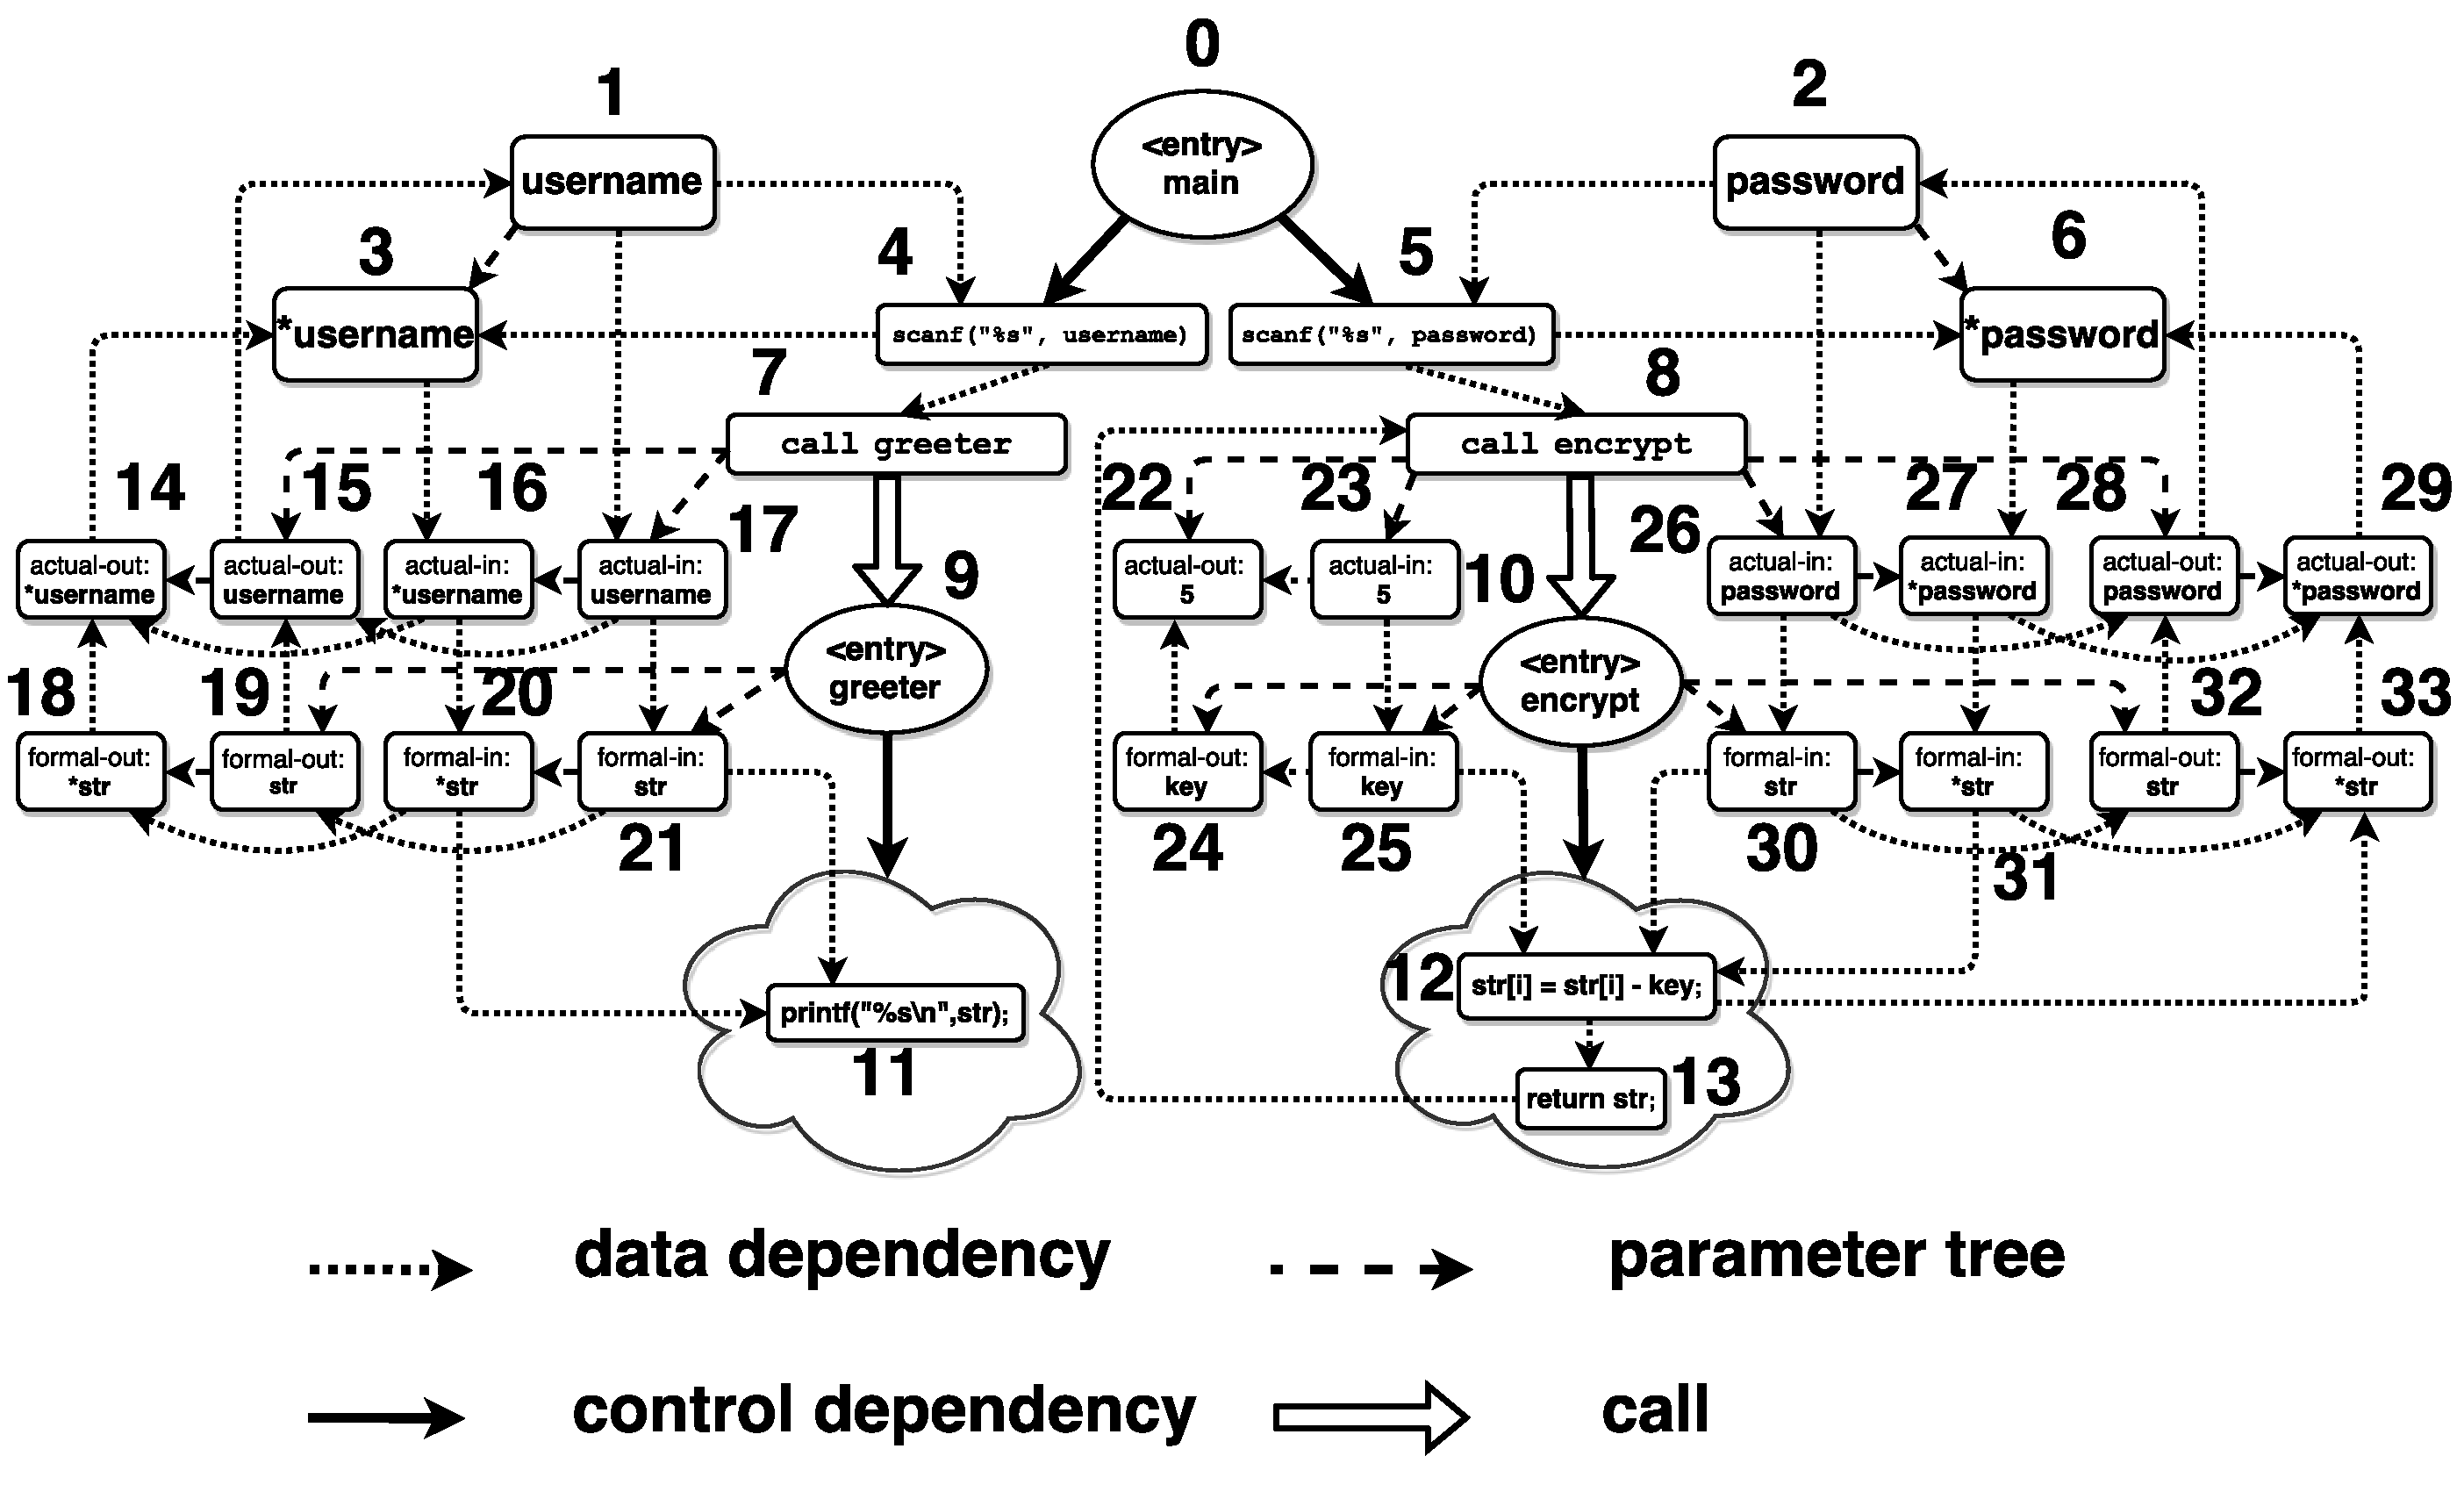
\includegraphics[width=\textwidth]{PDG.pdf}
%	%\vspace{-0.15in}
%	\caption{The program dependence graph of our toy program.}
%	\label{fig:daemon}
%	%\vspace{-0.2in}
%\end{figure}
%
%
%We use solid lines to represent the control dependences, and dotted lines to represent the data dependences. 
%
%The real difficulty is how to represent the inter-procedure data dependency. Out solution is using parameter trees, which 
%
%
%One problem when using parameter trees is elegantly deal with parameters with recursive data structures(e.g. linked list), which can lead to parameter trees of infinite depth. On this issue, we borrow the idea of J.~Graf's work\cite{objectgraph}. 
% ...
% 
%illustrate how cyclic(recursive) structures are accommodated by ... 
% 
% 
%linked list, tree...
% 




\begin{thebibliography}{1}

\bibitem{interslicing}
S. Horwitz, T. Reps, and D. Binkley. Interprocedural slicing using dependence graphs. In \emph{ACM Trans. Programming Languages and Systems}, vol. 12, no. 1, pages 35-46, 1990.



\bibitem{objectgraph}
J.~Graf. Speeding up context-, object- and
field-sensitive SDG generation. In \emph{Proc. 9th IEEE International Working Conference on Source Code Analysis and Manipulation}. IEEE Computer Society, pages 105-114, 2010.

\bibitem{k-limit}
D. Liang, M. J. Harrold. Slicing objects using system dependence graphs. In \emph{ICSM}, pages 358-367, 1998.


\bibitem{ferrante}
J. Ferrante, K.J. Ottenstein, and J.D. Warren. The program dependence graph and its use in optimization.In \emph{ACM Transactions on Programming Languages and Systems}, 9(3):319-349, 1987.

\bibitem{dsa}
C. Lattner, A. Lanharth, V. Adve. Making context-sensitive points-to analysis with heap cloning practical for the real world. In \emph{Proc. of PLDI}, 2007.

\bibitem{jujutsu}
I. Evans, F. Long, U. Otgonbaatar, H. Shrobe, M. Rinard, H. Okhravi, and S. Sidiroglou-Douskos. Control jujutsu: On the weaknesses of fine-grained control flow integrity.  In \emph{ACM SIGSAC Conference on Computer and Communications Security, CCS}, 2015.


%\relax 




\end{thebibliography}


 
\end{document}




















